
\subsubsection*{Rate of Decay}
\label{sec:findings-expts-decay}

%%%
In addition to the learning rate,
the decay parameter $d$ was also adjusted to see what sort of effect it
would have on learning.
%
Instead of the default decay rate of 10\%,
rates ranging from 0\% to 50\%
were tested to demonstrate the effect of temporal learning.
%%%

\paragraph*{Results}

%%%
% TODO: results
%%%

\begin{figure}[h]
	\centering

	\begin{tabular}{c | l l l l}
		% Outline:
		%   s\g |  250k | 500k | 750k | 1mm
		%   0.00
		%   0.10
		%   0.25
		%   0.50
		$d$ \textbf{\textbackslash} game & 250,000 & 500,000 & 750,000 & 1,000,000 \\
		\hline
		\\
		0.00 &
			\parbox[c]{5em}{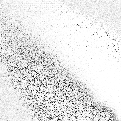
\includegraphics[width=\stratgraphwidthsmall]{images/findings/experiments/decay/decay_000_250.png}} & % 250
			\parbox[c]{5em}{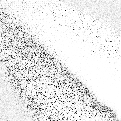
\includegraphics[width=\stratgraphwidthsmall]{images/findings/experiments/decay/decay_000_500.png}} & % 500
			\parbox[c]{5em}{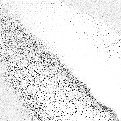
\includegraphics[width=\stratgraphwidthsmall]{images/findings/experiments/decay/decay_000_750.png}} & % 750
			\parbox[c]{5em}{
\includegraphics[width=\stratgraphwidthsmall]{images/findings/experiments/decay/decay_000_1mm.png}} \\ % 1mm
		\\
		0.10 & 
			\parbox[c]{5em}{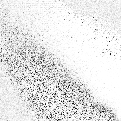
\includegraphics[width=\stratgraphwidthsmall]{images/findings/experiments/decay/decay_010_250.png}} & % 250
			\parbox[c]{5em}{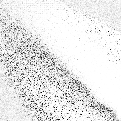
\includegraphics[width=\stratgraphwidthsmall]{images/findings/experiments/decay/decay_010_500.png}} & % 500
			\parbox[c]{5em}{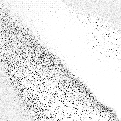
\includegraphics[width=\stratgraphwidthsmall]{images/findings/experiments/decay/decay_010_750.png}} & % 750
			\parbox[c]{5em}{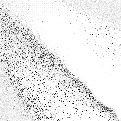
\includegraphics[width=\stratgraphwidthsmall]{images/findings/experiments/decay/decay_010_1mm.png}} \\ % 1mm
		\\
		0.25 & 
			\parbox[c]{5em}{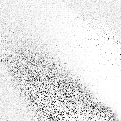
\includegraphics[width=\stratgraphwidthsmall]{images/findings/experiments/decay/decay_025_250.png}} & % 250
			\parbox[c]{5em}{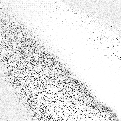
\includegraphics[width=\stratgraphwidthsmall]{images/findings/experiments/decay/decay_025_500.png}} & % 500
			\parbox[c]{5em}{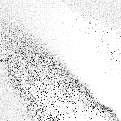
\includegraphics[width=\stratgraphwidthsmall]{images/findings/experiments/decay/decay_025_750.png}} & % 750
			\parbox[c]{5em}{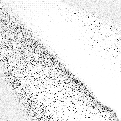
\includegraphics[width=\stratgraphwidthsmall]{images/findings/experiments/decay/decay_025_1mm.png}} \\ % 1mm
		\\
		0.50 & 
			\parbox[c]{5em}{
\includegraphics[width=\stratgraphwidthsmall]{images/findings/experiments/decay/decay_050_250.png}} & % 250
			\parbox[c]{5em}{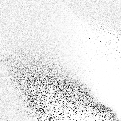
\includegraphics[width=\stratgraphwidthsmall]{images/findings/experiments/decay/decay_050_500.png}} & % 500
			\parbox[c]{5em}{
\includegraphics[width=\stratgraphwidthsmall]{images/findings/experiments/decay/decay_050_750.png}} & % 750
			\parbox[c]{5em}{
\includegraphics[width=\stratgraphwidthsmall]{images/findings/experiments/decay/decay_050_1mm.png}} \\ % 1mm
	\end{tabular}

\caption{
	Comparison of different decay rates learning the \handmaxavg\ strategy
	when playing as the dealer
	over the course of one million games.
	}
\label{fig:expts-decay-comp}
\end{figure}


